\documentclass{beamer}
\usepackage[utf8]{inputenc}

\usetheme{AnnArbor}
\usecolortheme{whale}
\usepackage{tabularx}
\usepackage{rotating,multirow}
\usepackage{float}

\definecolor{beamer@blendedblue}{rgb}{0.2,0.2,0.7} % use structure theme to change
\setbeamercolor{alerted text}{fg=red!85!black}
\setbeamercolor{frametitle}{bg=beamer@blendedblue}
\useinnertheme{rectangles}
\setbeamercolor{block title}{use=structure,fg=white,bg=structure.fg!75!black}
\setbeamercolor{block body}{parent=normal text,use=block title,bg=block title.bg!10!bg}

\setbeamertemplate{navigation symbols}{}
\setbeamertemplate{footline}{}

\title %optional
{Extracting and Exploring Information about Flood Events from Twitter}

% \author % (optional, for multiple authors)
% {Yasser Kaddoura}

\institute[VFU] % (optional)
{
  % Department of Information Technology\\
  % Uppsala University
  % \\[5mm]
  % Supervisors:\\
  % Carlo Navarra\inst{1},
  % Katerina Vrotsou\inst{2},
  % Kostiantyn Kucher\inst{2} \\
  % \inst{1,2}%
  % Linköping University,
  % \inst{1}%
  % Department of Thematic Studies, \\
  % \inst{2}%
  % Department of Science and Technology\\

}

\date % (optional)
% {Thesis Defence\\ April 20, 2023}

% \logo{
\includegraphics[height=1cm]{./images/UU_LOGO.png}}
\begin{document}

\frame{\titlepage

  \setbeamertemplate{headline}{}
}

% \begin{frame}
%   \frametitle{Contents}
%   \tableofcontents
% \end{frame}

\section{Research Questions and Significance}

\begin{frame}
  \frametitle{Research Questions}
  \begin{itemize} 
    \item How to classify relevant tweets?
    \item How to extract locations from tweets?
    \item What insights can be extracted from tweets' text?
    \item What visualizations can be used to represent the results? 
  \end{itemize}
\end{frame}

\begin{frame}
  \frametitle{Disaster management}
  \begin{columns}[T]
    \column{.5\textwidth}
    % Your image included here
    \begin{figure}
      \includegraphics[width=.7\textwidth]{./images/Flood_in_Pakistan_2022.png}
      \caption{Floods in Pakistan 2022\footnotemark}
    \end{figure}
  \pause
    \column{.5\textwidth}
  How can it facilitate disaster management?
  \begin{itemize}
    \item Preparation
    \item Response
    \item Recovery
  \end{itemize}
  \end{columns}
  \footnotetext[1]{https://en.wikipedia.org/wiki/2022\_Pakistan\_floods}
\end{frame}


\section{Methods}
\subsection{Data Collection \& Classification}
\begin{frame}[t]

  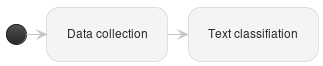
\includegraphics[scale=0.4]{./images/p1.png}

  \begin{itemize}

    \item \textbf{Unlabelled data}: 
      \begin{itemize}
    \item Extracted from Twitter API using flood relevant terms 
    \item Analyse historical flood events
      \end{itemize}
    \item \textbf{Labelled data}:  
      \begin{itemize}
        \item Crowdsourced datasets  (25000 tweets)
        \item Train DistilBERT to classify relevant tweets
      \end{itemize}
  \end{itemize}
\end{frame}

\subsection{Location Extraction \& Text Analysis}
\begin{frame}[t]

  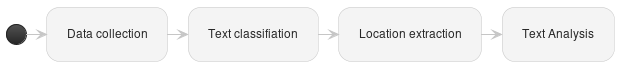
\includegraphics[scale=0.4]{./images/p3.png}

  \begin{itemize}
    \item Geoparsing process:
      \begin{itemize}
        \item \textbf{Toponym recognition} using an NER model
        \item \textbf{Toponym resolution} using OpenStreepMap
        \item Given two or more locations in one tweet, select the location with the smallest bounding box
      \end{itemize}

\item Text analysis techniques:
      \begin{itemize}
        \item Topic modelling using \textbf{LDA}
        \item Words relevance using \textbf{TF-IDF}
        \item Dimensionality reduction using \textbf{t-SNE} on TF-IDF matrix with DBSCAN clustering
      \end{itemize}
  \end{itemize}
\end{frame}
% \subsection{Text Analysis}
% \begin{frame}[t]
% \end{frame}

\subsection{Visualization}

\begin{frame}
  % \frametitle{Visualization}

  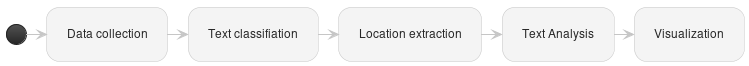
\includegraphics[scale=0.4]{./images/p4.png}
  \begin{figure}
    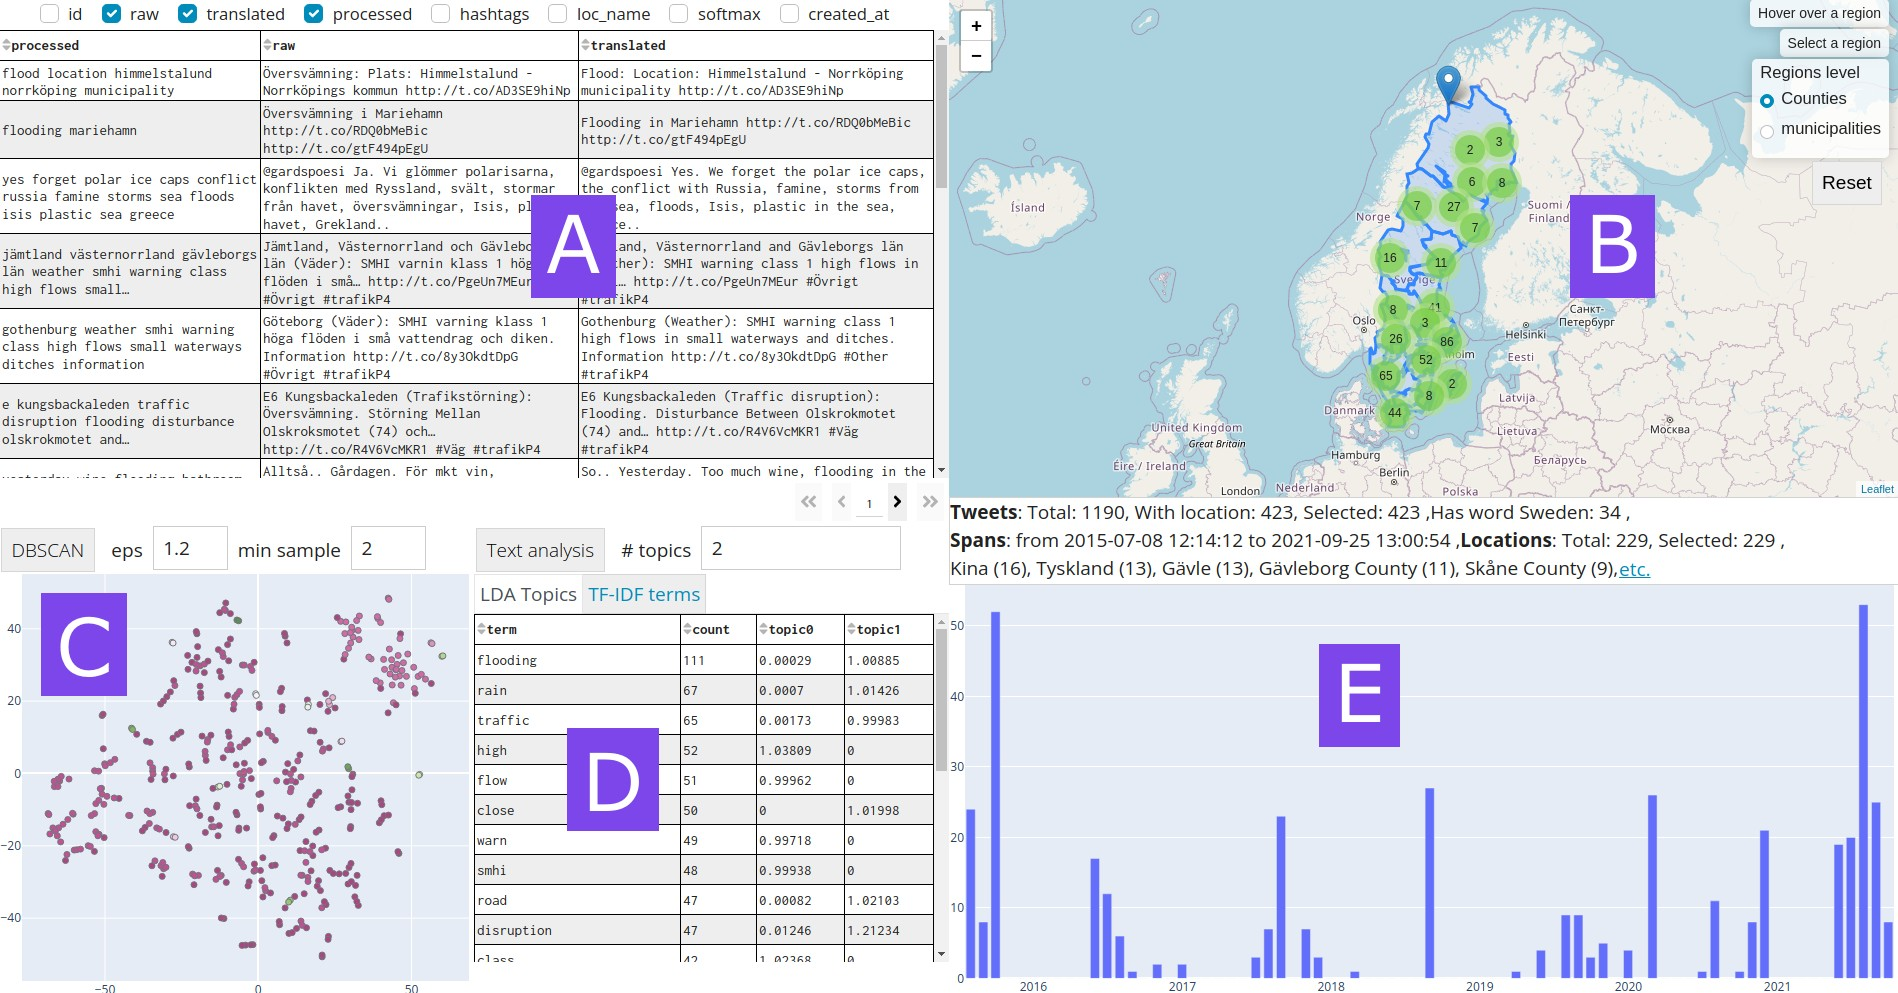
\includegraphics[width=\textwidth]{../report/images/visual_interface.png}
    \caption{Visual interface}
  \end{figure}
\end{frame}

% \begin{frame}
%   \begin{figure}
%     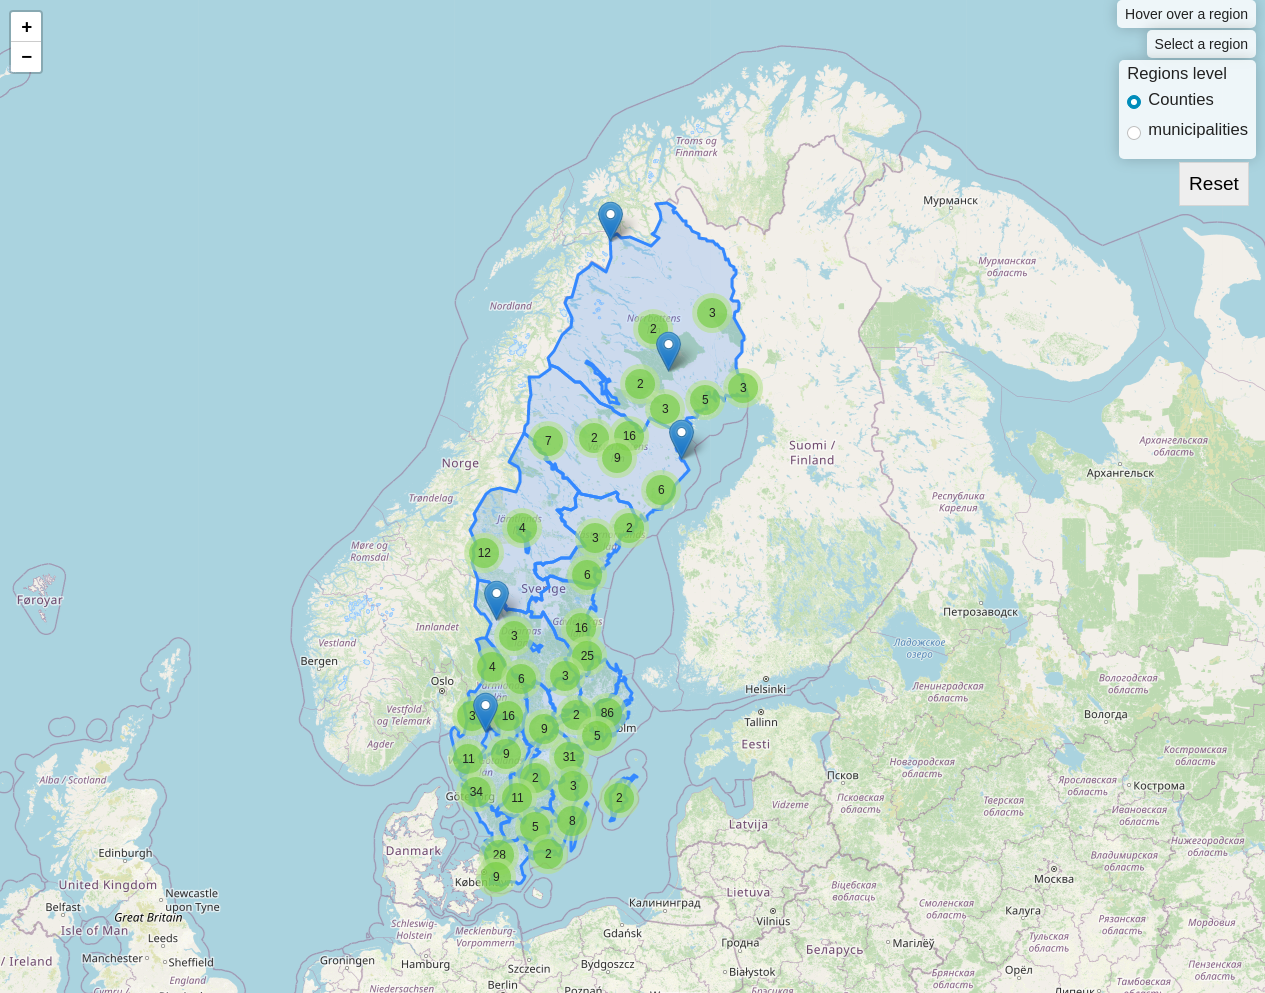
\includegraphics[height=0.85\textheight]{../report/images/map.png}
%     \caption{Map showing clusters of tweets}
%   \end{figure}
% \end{frame}

% \begin{frame}
%   \begin{figure}
%     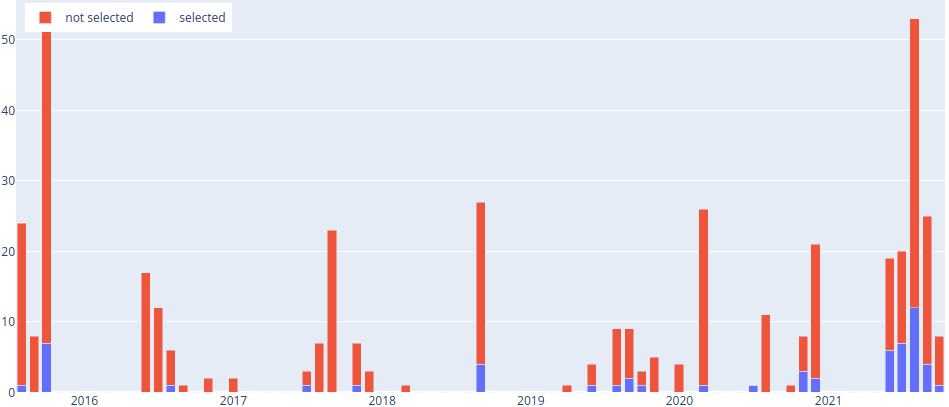
\includegraphics[width=\textwidth]{../report/images/histogram.png}
%     \caption{Histogram for tweets' creation dates}
%   \end{figure}
% \end{frame}

% \begin{frame}
%   \begin{figure}
%     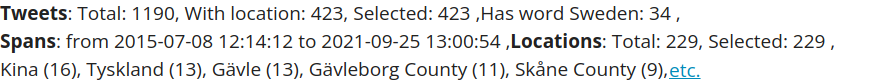
\includegraphics[width=\textwidth]{../report/images/meta_data.png}
%     \caption{Metadata about the tweets}
%   \end{figure}
%   \begin{figure}
%     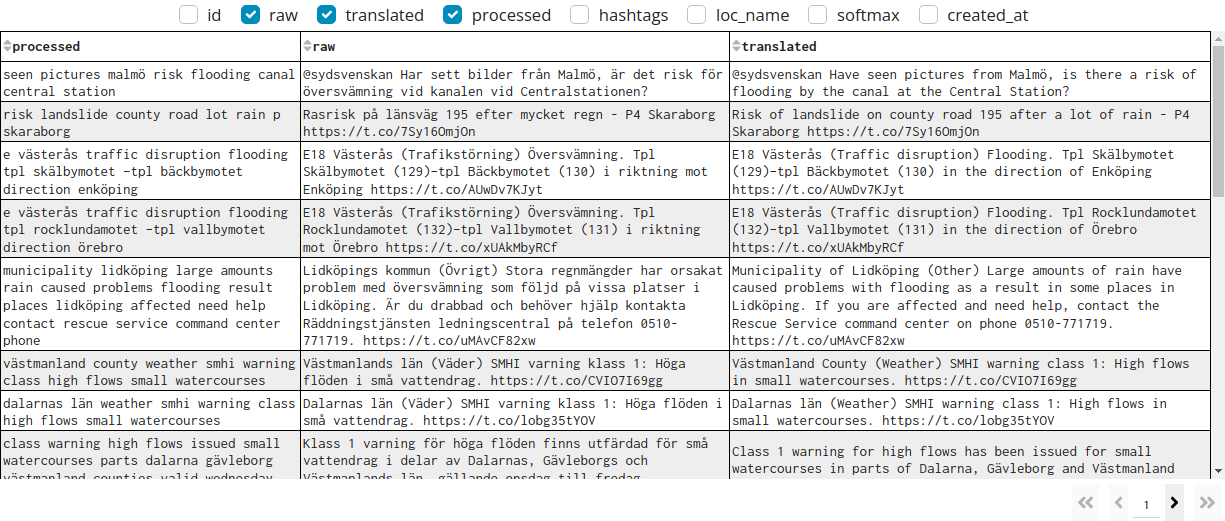
\includegraphics[width=\textwidth]{./images/tweets_table.png}
%     \caption{Tweets' table}
%   \end{figure}
% \end{frame}

% \begin{frame}
%   \begin{figure}
%     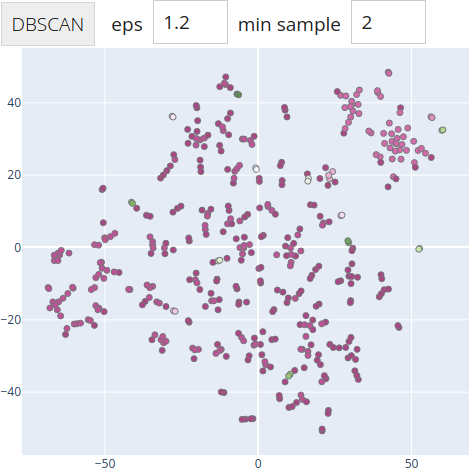
\includegraphics[width=0.5\textwidth]{../report/images/scatter.png}
%     \caption{Scatter plot for t-SNE's space}
%   \end{figure}
% \end{frame}

% \begin{frame}
%   \begin{columns}[T]
%     \column{.5\textwidth}
%     \begin{figure}
%       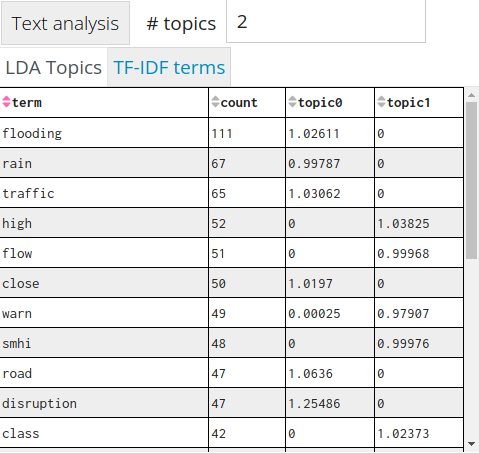
\includegraphics[width=\textwidth]{../report/images/lda_topics.png}
%       \caption{LDA topic weights}
%     \end{figure}
%     \column{.5\textwidth}
%     \begin{figure}
%       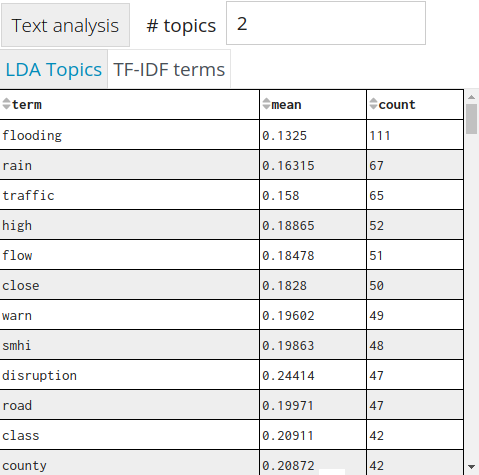
\includegraphics[width=\textwidth, trim={0 0.5cm 0 0},clip]{../report/images/tf_idf.png}
%       \caption{TF-IDF weights}
%     \end{figure}
%   \end{columns}
% \end{frame}


% \section{Pipeline Validation}
% \begin{frame}
%   \frametitle{Classifier Performance}
%   \begin{itemize}
%     \item Trained on 20,000 tweets
%     \item The metrics show that the trained classifier is performing well
%   \end{itemize}
%   \vspace{0.5cm}
% \begin{table}[H]
%   \center
%   \caption{Evaluation metrics}
%   \bgroup
%   \def\arraystretch{1.5}
%   \begin{tabular}{|c|c|c|c|c|}
%     \hline
%             Accuracy & Precision & Recall & F$_1$ Score & Confusion Matrix\\
%             \hline
%   0.9231 & 0.8944 & 0.9181 & 0.9061 &
%     $
%     \begin{bmatrix}
%       381 & 34 \\ 
%       45 & 568 
%     \end{bmatrix}
%     $\\
%     \hline
%   \end{tabular}
%   \egroup
% \end{table}

% \end{frame}

% \begin{frame}[t]
%   \frametitle{Experiment to validate the pipeline}
%   Extract one week's worth of tweets about a past flood event in Sweden:
%   \begin{itemize}
%     \item Flood event in Gävleborg and Dalarna counties on 18 August 2021
%     \item 1589 tweets from Twitter API
%     \item 910 left after pre-processing 
%     \item 700 classified as flood-relevent
%     \item 247 mentions locations
%     \item 96 mentions Gävle
%   \end{itemize}
% \end{frame}
% \newcolumntype{L}[1]{>{\raggedright\arraybackslash}p{#1}}
% \begin{frame}
%   \frametitle{Misclassified Tweets \& Misidentified Locations}
% \begin{table}
%   \center
%   \caption{Misclassified tweets for floods in Gävleborg and Dalarna}
%   \begin{tabular}{|L{5cm}|L{5cm}|}
%     \hline
%     Original tweet & Translated tweet\\
%     \hline
%     Blött i Gävle sa Bull.. https://t.co/fV1ChW7ZTR &
%     Wet in Gävle said Bull.. https://t.co/fV1ChW7ZTR \\
%     \hline
%     Nån som vet om det är lite blött i Gävle?&
%     Anyone know if it's a bit wet in Gävle? \\
%     \hline
%     Att tänka på mycket regn bakåt i tiden o tänka på bl.a. ån i Halland som steg o ställde till det !&
%     Thinking about a lot of rain back in time and thinking about e.g. the river in Halland that rose and
%     made it happen! \\
%     \hline
%   \end{tabular}
% \end{table}
% \end{frame}

\begin{frame}[t]
  \frametitle{Experiment to validate the pipeline}

  Classifier's accuracy (0.92), precision (0.9), recall (0.92) - trained on 20,000 tweets.

   \vspace{0.5cm}

  Extract one week's worth of tweets about a past flood event for a past event in 
  Gävleborg and Dalarna counties on 18 August 2021
\begin{itemize}
  \item \textbf{Misclassified Tweet}: A basement was flooded when a water main leaked in \#Vårberga in \#Borgå \#borgåvatten
  \item \textbf{Misidentified location}: Dödssiffran stiger i turkiska översvämningar
    \#\textbf{\alert{Turkiet}} \#svpol
    https://t.co/K6kLRmxQdw \\
    \textbf{Identified location}: Turkiet, a hamlet\footnote{isolated settlement} in Uppsala county. \\
    \textbf{Actual location}: Turkey, the country.
  % \item \textbf{Original tweet}: Information. Det kraftiga regnovädret över \textbf{\alert{Gävle}} har orsakat
  %   översvämningar i arenan. Detta innebär att all verksamhet i Monitor ERP \textbf{\alert{Arena}}, vilket inkluderar
  %   bland annat aktivitet på isen samt restaurangverksamheten, tills vidare är pausad. Vi återkommer
  %   med mer information. https://t.co/gHDfirq9VS \\
  %   \textbf{Identified location}: Årena, an isolated dwelling\footnote{consist of not more than 2 households}
  %   in Kalmar county. \\
  %   \textbf{Actual location}: Gävle.
\end{itemize}
\end{frame}

 % \begin{frame}[t]
 %  \frametitle{Visualization (Map)}
% \begin{figure}[H]
 %  \begin{center}
 %    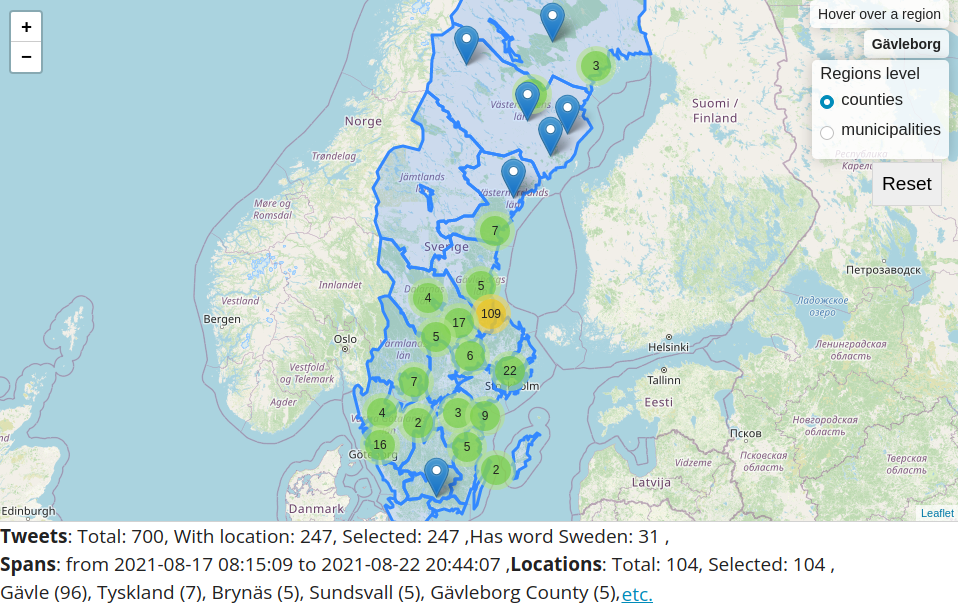
\includegraphics[height=0.7\textheight]{../report/images/gavle_map.png}
 %  \end{center}
 %  \caption{Map showing tweets about flood event in Gävleborg}
% \end{figure}
 % \end{frame}
 %  \begin{frame}[t]
 %    \frametitle{Visualization (Histogram)}
% \begin{figure}[H]
 %  \begin{center}
 %    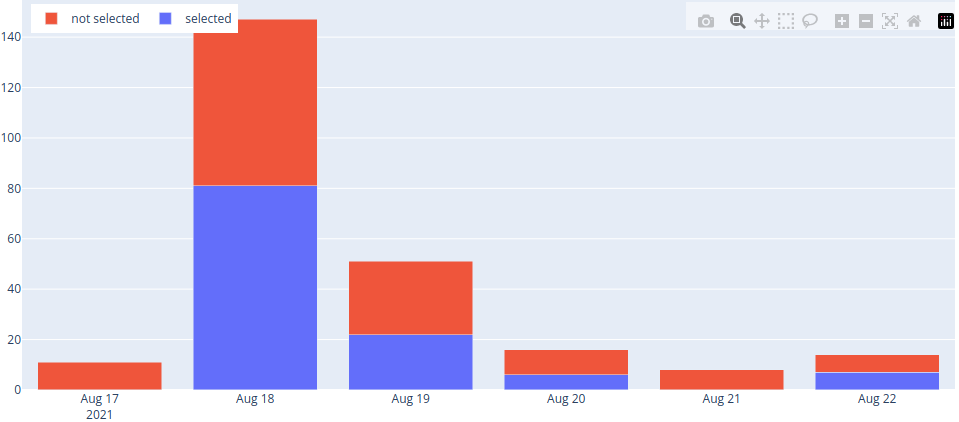
\includegraphics[width=\textwidth]{../report/images/gavle_histogram.png}
 %  \end{center}
 %  \caption{Histogram showing tweets about flood event in Gävleborg}
 %  \label{fig:gavle_histogram}
% \end{figure}
 %  \end{frame}

 %  \begin{frame}[t]
 %    \frametitle{Visualization (Text Analysis)}
% \begin{figure}[H]
 %  \begin{center}
 %    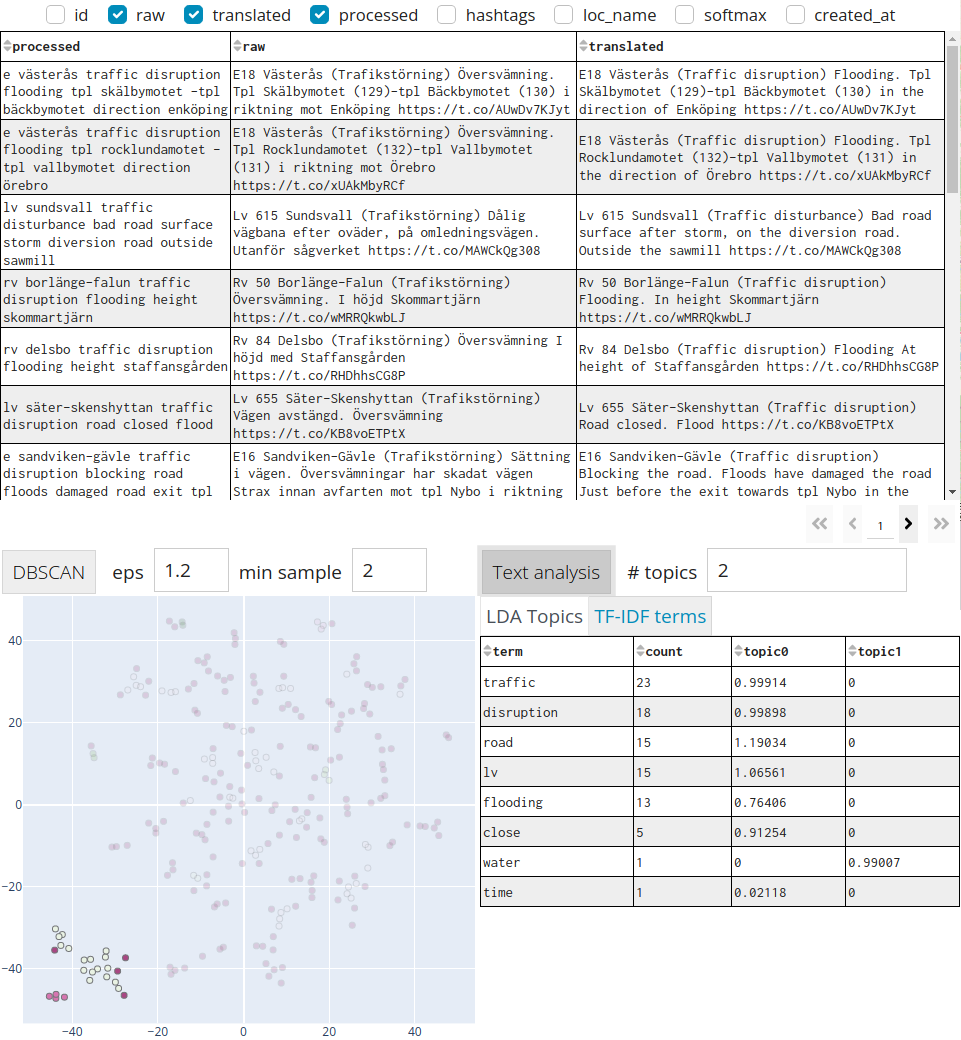
\includegraphics[width=0.9\columnwidth, trim={0cm 0cm 0cm 14.5cm},clip]{../report//images/gavle_text_analysis.png}
 %  \end{center}
 %  \caption{Scatter plot and LDA table showing a cluster of tweets about flood event in Gävleborg}
% \end{figure}
    
 %  \end{frame}

  \begin{frame}
\begin{center}
\Huge Short Demo
\end{center}
  \end{frame}
\section{Results Interpretation, Limitations and Future Work}

\begin{frame}
  \frametitle{Results Interpretation, Limitation and Future Word}
  \begin{itemize}
    \item Add more data sources
      \begin{itemize}
      \item Other social media platforms
      \item Media outlets 
      \item Meteorological data
      \end{itemize}
   % \item Spambot and fake news 
   \item Classifier performance
     \begin{itemize}
     \item Process other elements, such as Images and URLs
     \end{itemize}
   \item Identifying geographical locations
      \begin{itemize}
    \item Heuristics to identify correct location
      \end{itemize}
   % \item Visual interface
   %    \begin{itemize}
   %  \item Add more filtering options (e.g. text, LDA topics)
   %    \end{itemize}
    \item Future Work
    \begin{itemize}
      \item Forecasting 
      \item Other types of disasters
      \item Other countries
    \end{itemize}
  \end{itemize}
\end{frame}
\section{Summary and Last Words}
\begin{frame}[t]
  \frametitle{Summary and Last Words}
\begin{itemize}
  \item The pipeline is able to extract information about historical flood events
  \item Social media is a potential data source to augment disaster management pipelines but not as a
    standalone source
  \item Highly dependent on people's participation
  \item Potential framework acknowledged by the people to motivate them to share their knowledge
\end{itemize}
\end{frame}

\end{document}
